\section{Conduzione stazionaria}
Si ricordano le equazioni di Maxwell nel limite stazionario
considerando le leggi dell'elettrostatica unite a quella della
conservazione della carica 
$$
\oiint_{\Sigma} \vec{D}\cdot \hat{n} dS = Q_{lib}\ 
\forall\ \Sigma \ \text{Legge di Gauss}
$$
$$
\oint_{\Sigma}\vec{E}\cdot\hat{t} dl = 0 \ \forall\ \Gamma\ \ 
\text{Farady-Neumann}
$$
$$
\oiint_{\Sigma} \vec{J}\cdot\hat{n}dS = 0\ \ \forall\ \Sigma\
 \text{Principio di conservazione della carica}
$$
Si vedrà che una volta determinato il campo elettrico mediante
la sua funzione potenziale, ossia con problemi di valori al
contorno, si potranno facilmente determinare distribuzioni
di carica libera nei materiali e nei conduttori.

Dalle equazioni sopra riportate si vede che il campo
$\vec{J}$ è solenoidale mentre il campo $\vec{E}$ è 
conservativo.

\subparagraph{Conduttori ohmici}
Sia una regione $\Omega$ contenente un volumetto $\Delta\Omega$
di centro $P$, si chiama conduttore ohmico se rispetta la legge
di Ohm in forma locale 
$$
\vec{J}(P,t) = \gamma(P)\cdot\vec{E}(P,t) \Leftrightarrow \vec{E} = \eta\vec{J}
$$
$\gamma$ può essere una matrice se il materiale non è anisotropo, 
come quelli che sfruttano l'\href{https://it.wikipedia.org/wiki/Effetto_Hall}{effetto Hall}
 
È utile ricordare la conducibilità del rame pari a \SI{10e7}{\siemens\per\meter} (T $=$ \SI{20}{\celsius}). I limiti di
questo modello sono:
\begin{align*}
\text{Conduttore ideale: }& \gamma\to\infty,\eta\to 0 \Rightarrow 
\vec{J}\neq 0, \vec{E} = 0 \\
\text{Isolante ideale: }& \gamma\to 0 ,\eta\to\infty \Rightarrow
\vec{J} =0, \vec{E}\neq 0
\end{align*}

\subparagraph{Conduttori in aria} I conduttori vengono spesso rappresentati
collegati a dei morsetti o terminali ($T^+,T^-$) con resistività nulla 
mentre sono circondati da ``aria'' a resistività infinita
\begin{figure}[H]
\centering
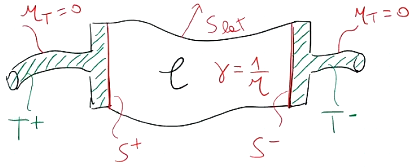
\includegraphics[width=0.5\linewidth]{modello_conduttore}
\end{figure}
Dato che il campo è necessariamente nullo in tutto il volume occupato
dai terminali, essi saranno equipotenziali.

La superficie esterna del conduttore invece, per rispettare il
principio di conservazione della carica rispetta la seguente
condizione in condizioni stazionarie
$$
\hat{n}\cdot\left(\vec{J}_2-\vec{J}_1\right) = 0
$$
Dove la regione 1 è quella del componente, la regione 2 è l'area
esterna, si può infatti porre $\vec{J}_2=0$ data la caratteristica
isolante dell'aria, ciò implica che \textbf{il vettore densità di corrente ha solo una componente tangenziale} alla superficie del conduttore
oppure che il conduttore è un tubo di flusso per il campo densità di 
corrente.

Fatta questa premessa si trova una condizione al contorno per il 
potenziale, ossia che la derivata normale sulla superficie laterale
per la funzione potenziale è nulla.
$$
\vec{J} = \gamma\vec{E} = -\gamma\nabla V \Rightarrow -\vec{J}_1\cdot
\hat{n} = \gamma \frac{\partial V_1}{\partial n} = 0
$$
Il potenziale sarà costante sulle superfici $S_1$ ed $S_2$ a causa
del potenziale sui morsetti, non varierà normalmente rispetto
alla superficie laterale, sono inoltre presenti anche due condizioni 
di Dirichlet, la soluzione esiste ed è unica.

\subparagraph{Circuito elementare con un generatore}
Si rappresentano due componenti collegati $C_1$ e $C_2$ e si 
rappresenta una linea $\Gamma$ chiusa orientata interna al circuito,
si applica la legge di Faraday-Neumann
\begin{figure}[H]
\centering
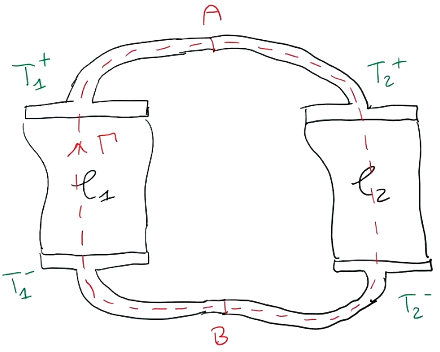
\includegraphics[width = 0.3\linewidth]{due_componenti_conduzione}
\end{figure}
$$
\oint_\Gamma\vec{E}\cdot\hat{t}dl = 0
$$
Nel caso generale ma se i materiali presenti in $C_1$ e $C_2$ sono
ohmici si avrà:
$$
\oint_\Gamma \eta\vec{J}\cdot\hat{t}dl = 0
$$
Il campo elettrico è quindi incapace di compiere lavoro affinché una 
carica di prova percorra quella linea chiusa, non ci può essere una 
corrente elettrica.

È necessario un campo ``elettromotore'' per stabilire la circolazione
di corrente, supposto per ipotesi nel conduttore $C_1$, ossia che
valga la relazione costitutiva
$$
\vec{J} = \gamma \left(\vec{E}+\vec{E}_m\right)
$$
dove $\vec{E}_m$ è il campo elettromotore di natura non puramente
elettrica (ad esempio elettro-chimica come una batteria).
Invertendo la precedente
$$
\vec{E} = \eta\vec{J} - \vec{E}_m
$$
Riscrivendo la legge di Faraday-Neumann
$$
\oint_{\Gamma}\vec{E}\cdot\hat{t}dl =  0 = \int_\Gamma \eta\vec{J}
\cdot\hat{t}dl - \int_\Gamma \vec{E}_m \cdot \hat{t}dl\Rightarrow
\int_\Gamma \vec{E}_m\cdot\hat{t}dl = \int_\Gamma \eta\vec{J}
\cdot\hat{t}dl
$$
L'integrale di linea del campo elettromotore viene indicato 
con
$\mathcal{E}$ e denominato ``forza elettromotrice'' lungo
la linea $\Gamma$, anche se dimensionalmente è un lavoro per unità
di carica e non una forza.

Se si assume il funzionamento a vuoto del circuito ossia $\vec{J} = 
0$, $C_1$ non collegato ad alcun componente 
\begin{figure}[H]
\centering
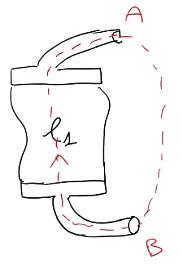
\includegraphics[width=0.3\linewidth]{generatore_a_vuoto}
\end{figure}
allora la F.E.M. è pari all'integrale 
$$
-\mathcal{E} = \oint_\Gamma \vec{E}\cdot\hat{t}dl \Rightarrow 
\mathcal{E} = \int_A^B \vec{E}\cdot\hat{t}dl = \left.v_{AB}\right|_{\Gamma_A}
$$
Dove $\Gamma_A$ è il tratto di circuitazione esterno al 
generatore.
La tensione a vuoto ai capi del generatore coincide proprio 
con la forza elettromotrice.

\subparagraph{Circuito elettrico}
Si vuole risolvere il problema di campo di corrente
stazionario nel seguente circuito
\begin{figure}[H]
\centering
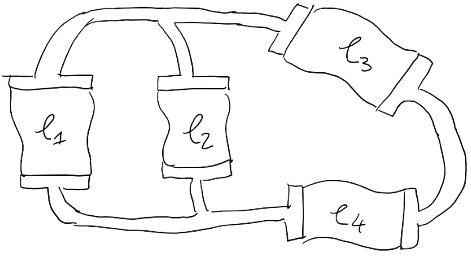
\includegraphics[width = 0.3\linewidth]{circuito_conduzione_stazionaria}
\end{figure}

Si considera il k-esimo componente $C_k$ collegato ai terminali $(r)$ ed $(s)$
detti anche nodi, essi saranno regioni equipotenziali.
\begin{figure}[H]
\centering
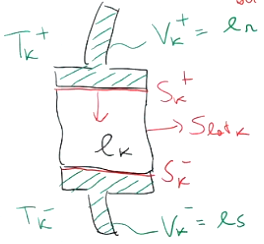
\includegraphics[width = 0.3\linewidth]{conduttore_singolo}
\end{figure}
Ricordando le equazioni della conduzione stazionaria
$$
\begin{aligned}
\nabla\cdot\vec{J} = 0 & \qquad \vec{J} = \gamma \vec{E} = -\gamma\nabla V\\
\vec{E} = -\nabla V & \qquad \nabla\cdot\left(-\gamma\nabla V\right) = 0 \Rightarrow \nabla^2 V = 0 \text{ nel materiale conduttore omogeneo}
\end{aligned}
$$
Nel conduttore il problema diventa
$$
\begin{cases}
\nabla^2 v &= 0  \text{ in } C\\
\left.V\right|_{S_k^+} &= e_r\\
\left.V\right|_{S_k^-} &= e_s\\
\left.\frac{\partial V}{\partial n}\right|_{S_{lat_k}} &= 0
\end{cases}
$$
Questo problema è ben posto e ammette soluzione unica, introduciamo una soluzione 
fondamentale 
$$
V^{(k)}: \begin{cases}
\nabla^2 V^{(k)} &= 0 \text{ in } C_k\\
V^(k) &= 1 \text{ su } S_k^+ \\
V^(k) &= 0 \text{ su } S_k^- \\
\frac{\partial V^{(k)}}{\partial n} &= 0 \text{ su } S_{lat_k}
\end{cases}
k = 1,...,l
$$
con $l$ il numero di bipoli. La soluzione del problema originario si ottiene con il
principio di sovrapposizione degli effetti:
$$
V = \sum_{k=1}^l a_kV^{(k)} \Rightarrow V(P) = (V_k^+ - V_k^-)V^{(k)}(P) + V_k^-
$$
Verifichiamo che questa sia proprio la soluzione ricordando che il Laplaciano 
di ogni singola funzione $V$ è nullo per ciascun bipolo
$$
\begin{aligned}
\nabla^2 V &= \nabla^2 V^{(k)} = 0\\
V|_{S_k^+} &= (V_k^+ - \cancel{V_K^-})\cdot 1 + \cancel{V_K^-} = V_k^+ \\
V|_{S_k^-} &= (V_k^+ - V_k^-)\cdot 0 + V_k^- = V_k^-
\end{aligned}
$$

Si considera ora una superficie $\Sigma$ composta dalla superficie $S_k^+$ e da una
superficie che taglia il terminale $(r)$ in aria, sia $S_r$ la parte di questa 
superficie che interseca il terminale, con normale entrante.
Se si applica il principio di conservazione della carica
$$
\oiint_\Sigma \vec{J}\cdot\hat{n} dS = 0 \Rightarrow i_{S_r} = i_{S_k^+} = \iint_{S_k} \vec{J}\cdot\hat{n}dS = \iint_{S_k^+}-\gamma\frac{\partial V}{\partial n} dS
$$
Sostituendo la soluzione di $V$ prima ottenuta
$$
i_{S_r} = i_k = \iint_{S_k^+} -\gamma\left(V_k^+ - V_k^-\right)\frac{\partial V}{\partial n}^{(k)} dS = \left( \iint_{S_k^+} -\gamma\frac{\partial V}{\partial n}^{(k)} dS \right)
v_k = G_k v_k
$$
dove $v_k$ è proprio la tensione ai capi del componente mentre il coefficiente $G_k$
tra parentesi è il rapporto tra una corrente e una tensione ossia una conduttanza.
Definendo $R_k = \frac{1}{G_k}$ si ottiene la legge di Ohm in forma integrale
ossia
$$
v_k = R_ki_k
$$

S si suppone che nel componente sia presente un campo elettromotore, con il PSE
si sommano le due tensioni
$$
\begin{cases}
v_k' = \mathcal{E} & \text{a vuoto}\\
v_k'' = R_ki_k 
\end{cases}\Rightarrow
v_k = v_k' + v_k'' = \mathcal{E} + R_ki_k
$$
Ossia l'equazione caratteristica di un generatore reale di tensione formato da uno ideale
con una resistenza in serie.
